\documentclass[border=8pt,tikz]{standalone}
\usepackage{tikz}
% Shared TikZ style for Chapter 5 diagrams.
% Inputted by every standalone diagram file.

\usetikzlibrary{
  arrows.meta,
  positioning,
  shapes.geometric,
  shapes.symbols,
  shapes.multipart,
  shapes.misc,
  fit,
  calc,
  backgrounds,
  decorations.pathmorphing,
  decorations.pathreplacing,
  patterns,
  shadows.blur,
}

% ─── Colour palette ──────────────────────────────────────────────
\definecolor{strixBlue}{HTML}{3B7DD8}     % data sources / inputs
\definecolor{strixGreen}{HTML}{22A699}    % processing / workers
\definecolor{strixOrange}{HTML}{E08036}   % storage
\definecolor{strixRed}{HTML}{E04B4B}      % attacker / external threat
\definecolor{strixPurple}{HTML}{6B5DD3}   % frontend / UI
\definecolor{strixGold}{HTML}{F2BE22}     % models / ML
\definecolor{strixGrey}{HTML}{6E7681}     % neutral / labels
\definecolor{strixDark}{HTML}{1F2933}     % titles / borders

% ─── Common node styles ──────────────────────────────────────────
\tikzset{
  >={Latex[width=2mm,length=2.5mm]},
  font=\sffamily\small,
  every node/.style={align=center},
  comp/.style={
    rectangle, rounded corners=2pt, draw=#1, fill=#1!10, very thick,
    text=strixDark, minimum width=22mm, minimum height=8mm,
    inner sep=4pt,
  },
  comp/.default=strixGreen,
  store/.style={
    cylinder, shape border rotate=90, aspect=0.3, draw=strixOrange,
    fill=strixOrange!12, very thick, text=strixDark,
    minimum width=18mm, minimum height=10mm, inner sep=2pt,
  },
  stream/.style={
    rectangle, rounded corners=2pt, draw=strixOrange,
    fill=strixOrange!8, dashed, thick, text=strixDark,
    minimum width=22mm, minimum height=7mm, inner sep=3pt,
    font=\ttfamily\scriptsize,
  },
  source/.style={comp=strixBlue},
  worker/.style={comp=strixGreen},
  model/.style={comp=strixGold},
  ui/.style={comp=strixPurple},
  ext/.style={comp=strixRed},
  title/.style={font=\sffamily\bfseries, text=strixDark},
  edge/.style={->, thick, draw=strixGrey, font=\sffamily\scriptsize\itshape},
  edgeStrong/.style={->, very thick, draw=strixDark, font=\sffamily\scriptsize\bfseries},
  group/.style={
    rectangle, rounded corners=4pt, draw=strixGrey, dashed, thick,
    inner sep=6pt, fill=strixGrey!4,
  },
  badge/.style={
    rectangle, rounded corners=1pt, fill=#1, text=white,
    font=\sffamily\scriptsize\bfseries, inner sep=2pt,
  },
  badge/.default=strixDark,
  port/.style={
    rectangle, rounded corners=1pt, draw=strixDark, fill=strixGrey!8,
    font=\ttfamily\scriptsize, minimum width=14mm, inner sep=2pt,
  },
}


\begin{document}
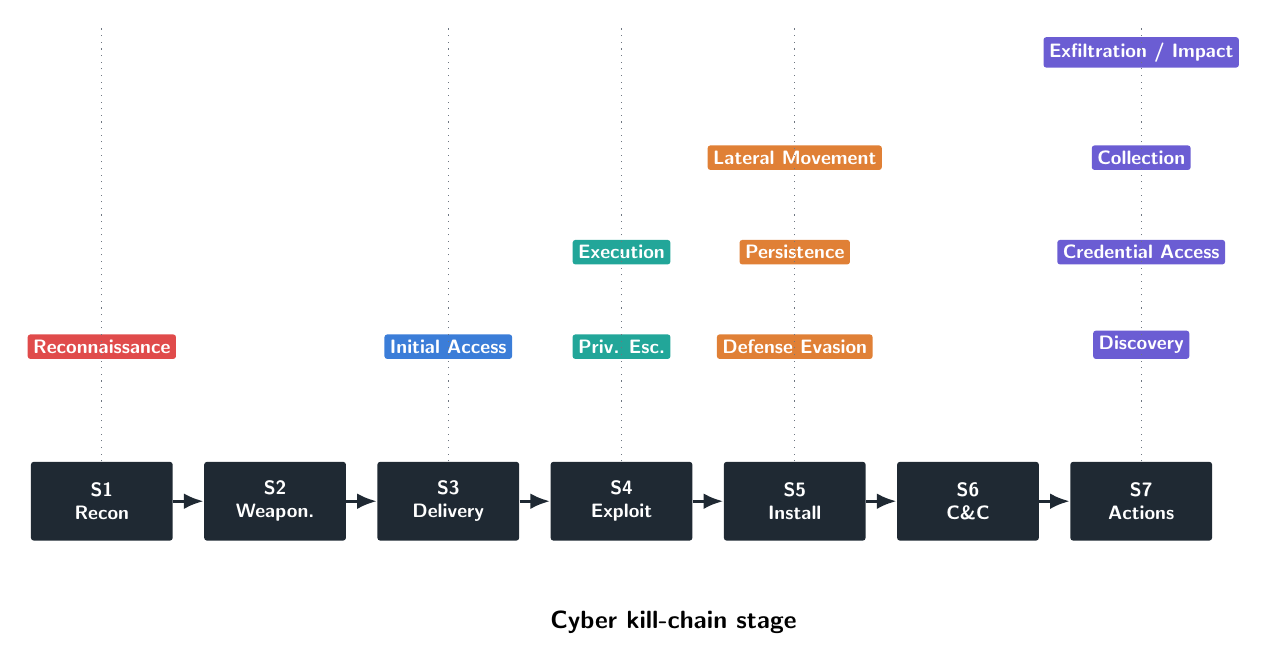
\begin{tikzpicture}[node distance=3mm]

% CKC spine
\def\stages{S1/Recon, S2/Weapon., S3/Delivery, S4/Exploit, S5/Install, S6/C\&C, S7/Actions}
\foreach \i/\pair in {0/S1\\Recon, 1/S2\\Weapon., 2/S3\\Delivery, 3/S4\\Exploit, 4/S5\\Install, 5/S6\\C\&C, 6/S7\\Actions} {
  \node[badge=strixDark, minimum width=18mm, minimum height=10mm, font=\sffamily\scriptsize\bfseries]
    at (\i*22mm, 0) (s\i) {\pair};
}
\foreach \i [evaluate=\i as \j using int(\i+1)] in {0,1,2,3,4,5} {
  \draw[->, very thick, draw=strixDark] (s\i.east) -- (s\j.west);
}

% Tactic chips above
\def\rowA{18mm}
\def\rowB{30mm}
\def\rowC{42mm}

% S1
\node[badge=strixRed, anchor=south] at ($(s0)+(0,\rowA)$) {Reconnaissance};

% S3
\node[badge=strixBlue, anchor=south] at ($(s2)+(0,\rowA)$) {Initial Access};

% S4
\node[badge=strixGreen, anchor=south] at ($(s3)+(0,\rowA)$) {Priv. Esc.};
\node[badge=strixGreen, anchor=south] at ($(s3)+(0,\rowB)$) {Execution};

% S5
\node[badge=strixOrange, anchor=south] at ($(s4)+(0,\rowA)$) {Defense Evasion};
\node[badge=strixOrange, anchor=south] at ($(s4)+(0,\rowB)$) {Persistence};
\node[badge=strixOrange, anchor=south] at ($(s4)+(0,\rowC)$) {Lateral Movement};

% S7
\node[badge=strixPurple, anchor=south] at ($(s6)+(0,\rowA)$) {Discovery};
\node[badge=strixPurple, anchor=south] at ($(s6)+(0,\rowB)$) {Credential Access};
\node[badge=strixPurple, anchor=south] at ($(s6)+(0,\rowC)$) {Collection};
\node[badge=strixPurple, anchor=south] at ($(s6)+(0,55mm)$) {Exfiltration / Impact};

% Dotted vertical mapping lines
\foreach \i in {0,2,3,4,6} {
  \draw[dotted, draw=strixGrey] (s\i.north) -- ++(0,55mm);
}

\node[font=\sffamily\bfseries\small, anchor=south] at (3.3*22mm,-18mm) {Cyber kill-chain stage};

\end{tikzpicture}
\end{document}
